\documentclass[10pt]{article}

% Set landscape mode and custom margins for page while including space for the footer
\usepackage[includefoot, margin={0.5cm, 0.5cm}, landscape]{geometry}

\usepackage{graphicx}

% Used to reduce the spacing around section headers and titles.
% Format title headers by adjusting font size
% Set the spacing on all sides of the title to 0
\usepackage[explicit]{titlesec}
\titleformat{\section}{\large\bfseries}{\thesection}{1em}{\underline{#1}}
\titleformat{\subsection}{\normalsize\bfseries}{\thesubsection}{1em}{#1}
\titleformat{\subsubsection}{\small\bfseries}{\thesubsubsection}{1em}{#1}
\titlespacing*{\section}{0pt}{*0}{0pt}
\titlespacing*{\subsection}{0pt}{*0}{0pt}
\titlespacing*{\subsubsection}{0pt}{*0}{0pt}

% Reduce spacing around list items
\usepackage{enumitem}
\setlist{nolistsep}

% Set line spacing
\usepackage{setspace}
\singlespacing

% Create a multicolumn layout
% Set the amount of separation between columns
% Draw a vertical rule between the columns
\usepackage{multicol}
\setlength{\columnsep}{1cm}
\setlength{\columnseprule}{0.1pt}

% Add a frame around the content
\usepackage{mdframed}

% Remove paragraph indent
\setlength{\parindent}{0pt}

% Custom footer (and header if I wanted)
\usepackage{fancyhdr}
\pagestyle{fancy}

% Set custom headers and footers for fancyhdr
\fancyhead{}
\fancyfoot[C]{Trajan Summary Sheet v1.0}
\renewcommand{\headrulewidth}{0pt} 	% Remove horizontal rule from header
\renewcommand{\footrulewidth}{0pt}  % Remove horizontal rule from footer

% Custom frame style for mdframed
% The negative margin is needed to fix a weird spacing that I couldn't figure out
\mdfdefinestyle{customFrame}{%
    outerlinewidth = 0.4pt,
    innertopmargin = -0.3cm}

% Reduce whitespace in the enumerate list environment
\newenvironment{enumerateCustom}
{\begin{enumerate}
  \setlength{\itemsep}{1pt}
  \setlength{\parskip}{0pt}
  \setlength{\parsep}{0pt}}
{\end{enumerate}}

% Reduce whitespace in the itemize list environment
\newenvironment{itemizeCustom}
{\begin{itemize}
  \setlength{\itemsep}{1pt}
  \setlength{\parskip}{0pt}
  \setlength{\parsep}{0pt}}
{\end{itemize}}

\begin{document}
\begin{multicols*}{2}

\section*{Setup}
    \begin{enumerateCustom}
        \item Set out main board. Give each player a board and all pieces of one color. 
        \item Place round tracker disc on circle for player count. 
        \item Place boat tiles in port color side up.
        \item Play 4 \textbf{quarter year} tiles ordered in a stack near board.
        \item Sort extra action (back) and Forum tiles (back), shuffle, and place face down piles near board
        \item Randomize demand tiles (circular blue green), remove 3 from game, and place stack face down near board.
        \item Place randomly 10 forum tiles in provinces at top of board (1 each).
        \item Place 6/9/12 forums tiles on designated Forum 
\includegraphics[scale=0.2]{images/forum.jpg} spaces for 2/3/4 players.
        \item Place 3 extra action tiles on yellow forum spaces.
        \item Fill all 20 spaces in Construction \protect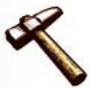
\includegraphics[scale=0.2]{images/construction.jpg} district with pentagon construction tiles (back)
        \item Each player places military leader and 1 player meeple on military camp (green oval) and 1 player meeple on work camp (red oval). Place remaining player meeples in top right area of play mat.
        \item Each player places 2 action markers in each tray on player mat.
        \item Sort Trajan tiles by category (icon) and place on 6 spaces on Trajan \protect
\includegraphics[scale=0.2]{images/trajan.jpg} district.
        \item Determine start player. Place player discs on Senate \protect
\includegraphics[scale=0.2]{images/senate.jpg} track start (blue circle). Start player token first, then next player's token on top, etc. Place player tokens on victory point track (order irrelevant).
        \item Draw 1 bonus per player from bag. Place by player board yellow side up.
        \item Draw 2 bonus tokens from bag and place on right of Senate track yellow side up.
        \item Shuffle commodity cards. Place pile face down by board. Reveal top two cards and create two discard piles on left and right of draw pile.
        \item In player order, each draws 3 commodity cards from any pile in any combination. If a discard pile is ever empty fill it with the top draw pile card.
        \item In player order, each picks 3 Trajan tiles. May only take 1 from each category. Place tiles on slots marked II, IV, and VI on player mat.
        \item Place Arch of Trajan on slot marked I.
    \end{enumerateCustom}

\section*{Gameplay}
Game is played over 4 \textbf{quarters} of a year. Each quarter consists of 4 \textbf{rounds}. Each lasts as long as one cycle of the time marker on the time track.

\section*{Player Turn}
A player's turn consists of the following steps in order:
    \begin{enumerateCustom}
        \item (mandatory) Rearrange action markers and move time marker
        \item (if possible) Accomplish Trajan tile
        \item (optional) Perform 1 action
    \end{enumerateCustom}

\subsection*{Rearrange action markers}
    \begin{enumerateCustom}
        \item Choose 1 tray on play mat. Take all action markers (must be at least 1). 
        \item Allocate each one in a tray in clockwise direction until all are allocated. The ending tray is the \textbf{target tray}. 
        \item Advance time marker equal to number of action markers selected from tray.
    \end{enumerateCustom}

\subsection*{Accomplish Trajan tile}
    Accomplish a Trajan if it is assigned to the \textbf{target tray} and there are action markers in the tray matching the colors shown on the tile. If so:
    \begin{itemizeCustom}
        \item Gain indicated victory points
        \item Optionally perform appropriate special action.
        \item Remove tile from game unless tile shows bread, helmet, or flame icon. Collect these on player mat.
    \end{itemizeCustom}

\subsection*{Perform One Action}
    Optionally perform the action indicated by the icon for the \textbf{target tray}.

\section*{Actions}
    \subsection*{\protect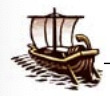
\includegraphics[scale=0.25]{images/seaport.jpg} Seaport}
    Choose 1 of 4 options:
    \begin{itemizeCustom}
        \item Draw 2 commodity cards from face down pile. Discard 1 card from hand.
        \item Draw top commodity card from one of the discard piles.
        \item Play 1 or 2 cards from hand face up in front of themselves. This is player's personal display. Draw number of played cards from face down draw pile.
        \item Ship commodities aboard 1 of 3 ships. Played cards go into personal display and combination must match requirement on one of ship tiles. Gain victory points indicated. Flip ship to gray back side if not flipped.
    \end{itemizeCustom}
    
    \subsection*{\protect
\includegraphics[scale=0.25]{images/forum.jpg} Forum}
    Take any 1 tile and place face up on designated space of player mat.

    \subsection*{\protect
\includegraphics[scale=0.25]{images/military.jpg} Military}
    Choose 1 of 3 options:
    \begin{itemizeCustom}
        \item Convert player meeting into legionnaire by moving meeple from player board to military camp.
        \item Move leader to adjacent province. Take tile if present and place on player mat.
        \item Relocate legionnaire from military camp to leader's province \textbf{if player's legionnaires aren't there}. Gain victory points indicated on province minus 3 per enemy legionnaire there.

    \end{itemizeCustom}

    \subsection*{\protect
\includegraphics[scale=0.25]{images/trajan.jpg} Trajan}
    Take top tile from 1 of 6 stacks and put on current Arch of Trajan slot. Slide Arch to next free slot in clockwise direction. If all are filled, put in center of action circle and relocate once a slot is free. Player can't take Trajan action if no slot is free.

    \subsection*{\protect
\includegraphics[scale=0.25]{images/senate.jpg} Senate}
    Advance disc on track by 1 space and gain indicated victory points. Active player puts disc on top of existing markers in space. Player can't take this action if marker is currently on 8 VP space.

    \subsection*{\protect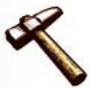
\includegraphics[scale=0.25]{images/construction.jpg} Construction}
    Choose 1 of 2 options:
    \begin{itemizeCustom}
        \item Convert player meeple into worker by moving meeple from player board to worker camp.
        \item Place one worker from worker camp into construction site. If first placement, pick any space in district. Otherwise, place orthogonally adjacent to 1 of their workers. Take tile in space if present, gain victory points, and place on indicated space on player mat. Workers may be deployed in location occupied by other player's worker.
            \begin{itemizeCustom}
            \item If first construction of type added to player mat, immediate perform assigned action in addition to ordinary turn.
            \end{itemizeCustom}
    \end{itemizeCustom}


\section*{End of Game Round}
The round ends when the time marker crosses its start space after the active player's turn. If there are less than 3 demand tiles revealed, reveal one and continue play. Otherwise, go to End of Year Quarter.

\section*{End of Year Quarter}
\begin{enumerateCustom}
    \item \textbf{Meeting people's demands:} Each player must meet the people's demands. For each revealed demand tile spend matching forum tile or use Trajan tile. Trajan tiles may only be used once per quarterly scoring. Lose 4/9/15 VPs for 1/2/3 unmet demands.
    \item \textbf{Balance of power in the senate:} Resolve standing in senate based on number of votes equal to number indicated on senate track plus numbers on all senate tiles on player mat. Most votes is \textbf{consul} and picks 1 of 2 bonus tiles. Keep yellow side up. Second most is \textbf{vice consul} and takes other bonus tile, gray side up. Break ties in favor of player high up track or disc that is stacked higher. Move all discs back to start space ordered lowest vote count at bottom to most at top.

    \item \textbf{Remove tiles:} Remove all forum tiles used to meet people's demands. Remove all claimed senate tiles (purple forum tiles with votes indicated) regardless if they were used or not. Remove all tiles from the forum.
    \item \textbf{Refill game board spaces:} Draw 2 new bonus tiles and place near senate yellow side up. Place forum tile in empty provinces without military leader or legionnaire. Refill all forum spaces with new forum tiles and yellow extra action tiles. Turn ships color side up and remove quarter year indicator from top of stack. If last was removed, go to End of Game.
\end{enumerateCustom}

\section*{End of Game}
Gain victory points as follows:
\begin{itemizeCustom}
    \item 1 VP per commodity card in hand
    \item 1 VP per worker in worker camp
    \item 1 VP per legionnaire in military camp
    \item 1 VP per Trajan tile on action circle
    \item 10 VP per set of 3 construction tiles with identical icon
    \item 20 VP per set of 4 construction tiles with identical icon
    \item Value of each bonus tile.
\end{itemizeCustom}

Winner is player with most victory points. Break tie in favor of person higher on senate track.

\section*{Misc.}
\subsection*{Extra Action Tiles}
After performing an action, may repeat an action by discarding matching extra action tile. If +2 marker assigned to that action, may repeat it a second time. Extra action tiles are removed from game when used, +2 markers are kept. Can only perform 1 extra action in this way per turn.

\end{multicols*}
\end{document}
